%%%%%%%%%%%%%%%%%%%%%%%%%%%%%%%%%%%%%%%%%%%%%%%%%%%%%%%%%%%%%%%%%%%%%%%%%%%%%%%%
%% SECTION
%%%%%%%%%%%%%%%%%%%%%%%%%%%%%%%%%%%%%%%%%%%%%%%%%%%%%%%%%%%%%%%%%%%%%%%%%%%%%%%%
\section{\textcolor{red}{Historia da música do samba}}\index{Música do samba}

O samba é uns dos gêneros musicais mais conhecidos no Brasil do século XXI;
entre estes gêneros mais populares, temos por exemplo, ao ``forró'' e ao ``Sertanejo'';
sendo que o samba se distingue entre eles, 
como a principal expressão popular da música brasileira \cite[pp. 47]{diniz2008almanaque}. 

\textcolor{red}{Pelo telefone\cite{musicapelotelefone}}

\subsection{\textcolor{red}{Quais são os estilos de música do samba?}}

\begin{description}
\item[Maxixe:] \cite[pp. 9]{musicasambavariasdef1} 
\item[Candomblés e macumbas:] \cite[pp. 9]{musicasambavariasdef1} 
\item[Cururú:] \cite[pp. 9]{musicasambavariasdef1} 
\item[Partido alto:] \cite[pp. 9]{musicasambavariasdef1} 
\item[Samba canção:] \cite[pp. 9]{musicasambavariasdef1} 
\item[Samba batucada:] \cite[pp. 9]{musicasambavariasdef1} 
\end{description}

\subsection{\textcolor{blue}{Quais são os estilos de dança que se enquadram na música do samba?}}
\label{subsec:estilosdedanca}
A resposta mais simples poderia ser que, uma pessoa ao ser livre e independente,
pode escolher expressar-se na dança, de forma natural, como esta saia de si mesmo.
Porem, entrando em assuntos mais técnicos, 
e de acordo com os padrões socialmente mais comuns de ser achados atualmente;
existe um grupo de estilos de danças, que por suas caraterísticas, 
são consideradas que se enquadram muito bem na música do samba.

Entre os estilos que se dançam a dois temos \cite[pp. 134]{perna2002samba}:
\begin{description}
\item[Samba de gafieira (dança):] É uma dança a dois, que pode ser dançada em todos os estilos de música de samba,
com excepção de: samba enredo (música), samba reggae (música), samba rock (música), marcha e maxixe (música) \cite[pp. 134]{perna2002samba}, para mais detalhes ver Seção \ref{subsec:gafieiradancaestilos}.

\item[Samba liso:] Se dança similarmente ao samba de gafieira, 
porem com um estilo mais elegante, sem ginga né passos de efeito;
se dança bem em : samba-canção, bossa nova e choro \cite[pp. 134]{perna2002samba}.

\item[Samba pagode:] É um estilo de dança a dois, originário de São Paulo, 
e é uma dança com poucos deslocamentos \cite[pp. 134]{perna2002samba}.

\item[Samba rock:] É um estilo de dança a dois, sendo esta uma dança variante das danças do swing/rock,
se dança bem em: samba rock (música), samba suingue e samba-funk \cite[pp. 135, 138]{perna2002samba}.

\item[Samba funkeado:] Também chamado estilo Jimmy de Oliveira, em honor a seu criador.

\item[Samba internacional:] É um estilo de dança a dois, influenciado pelo maxixe;
se dança principalmente fora do Brasil e existem basicamente dois estilos: 
o estilo internacional e o estilo norte-americano \cite[pp. 134-135]{perna2002samba}.

\end{description}

Figura \ref{fig:sambadavavsmusica} \cite[pp. 134-138]{perna2002samba}

\begin{figure}[h]
  \centering
    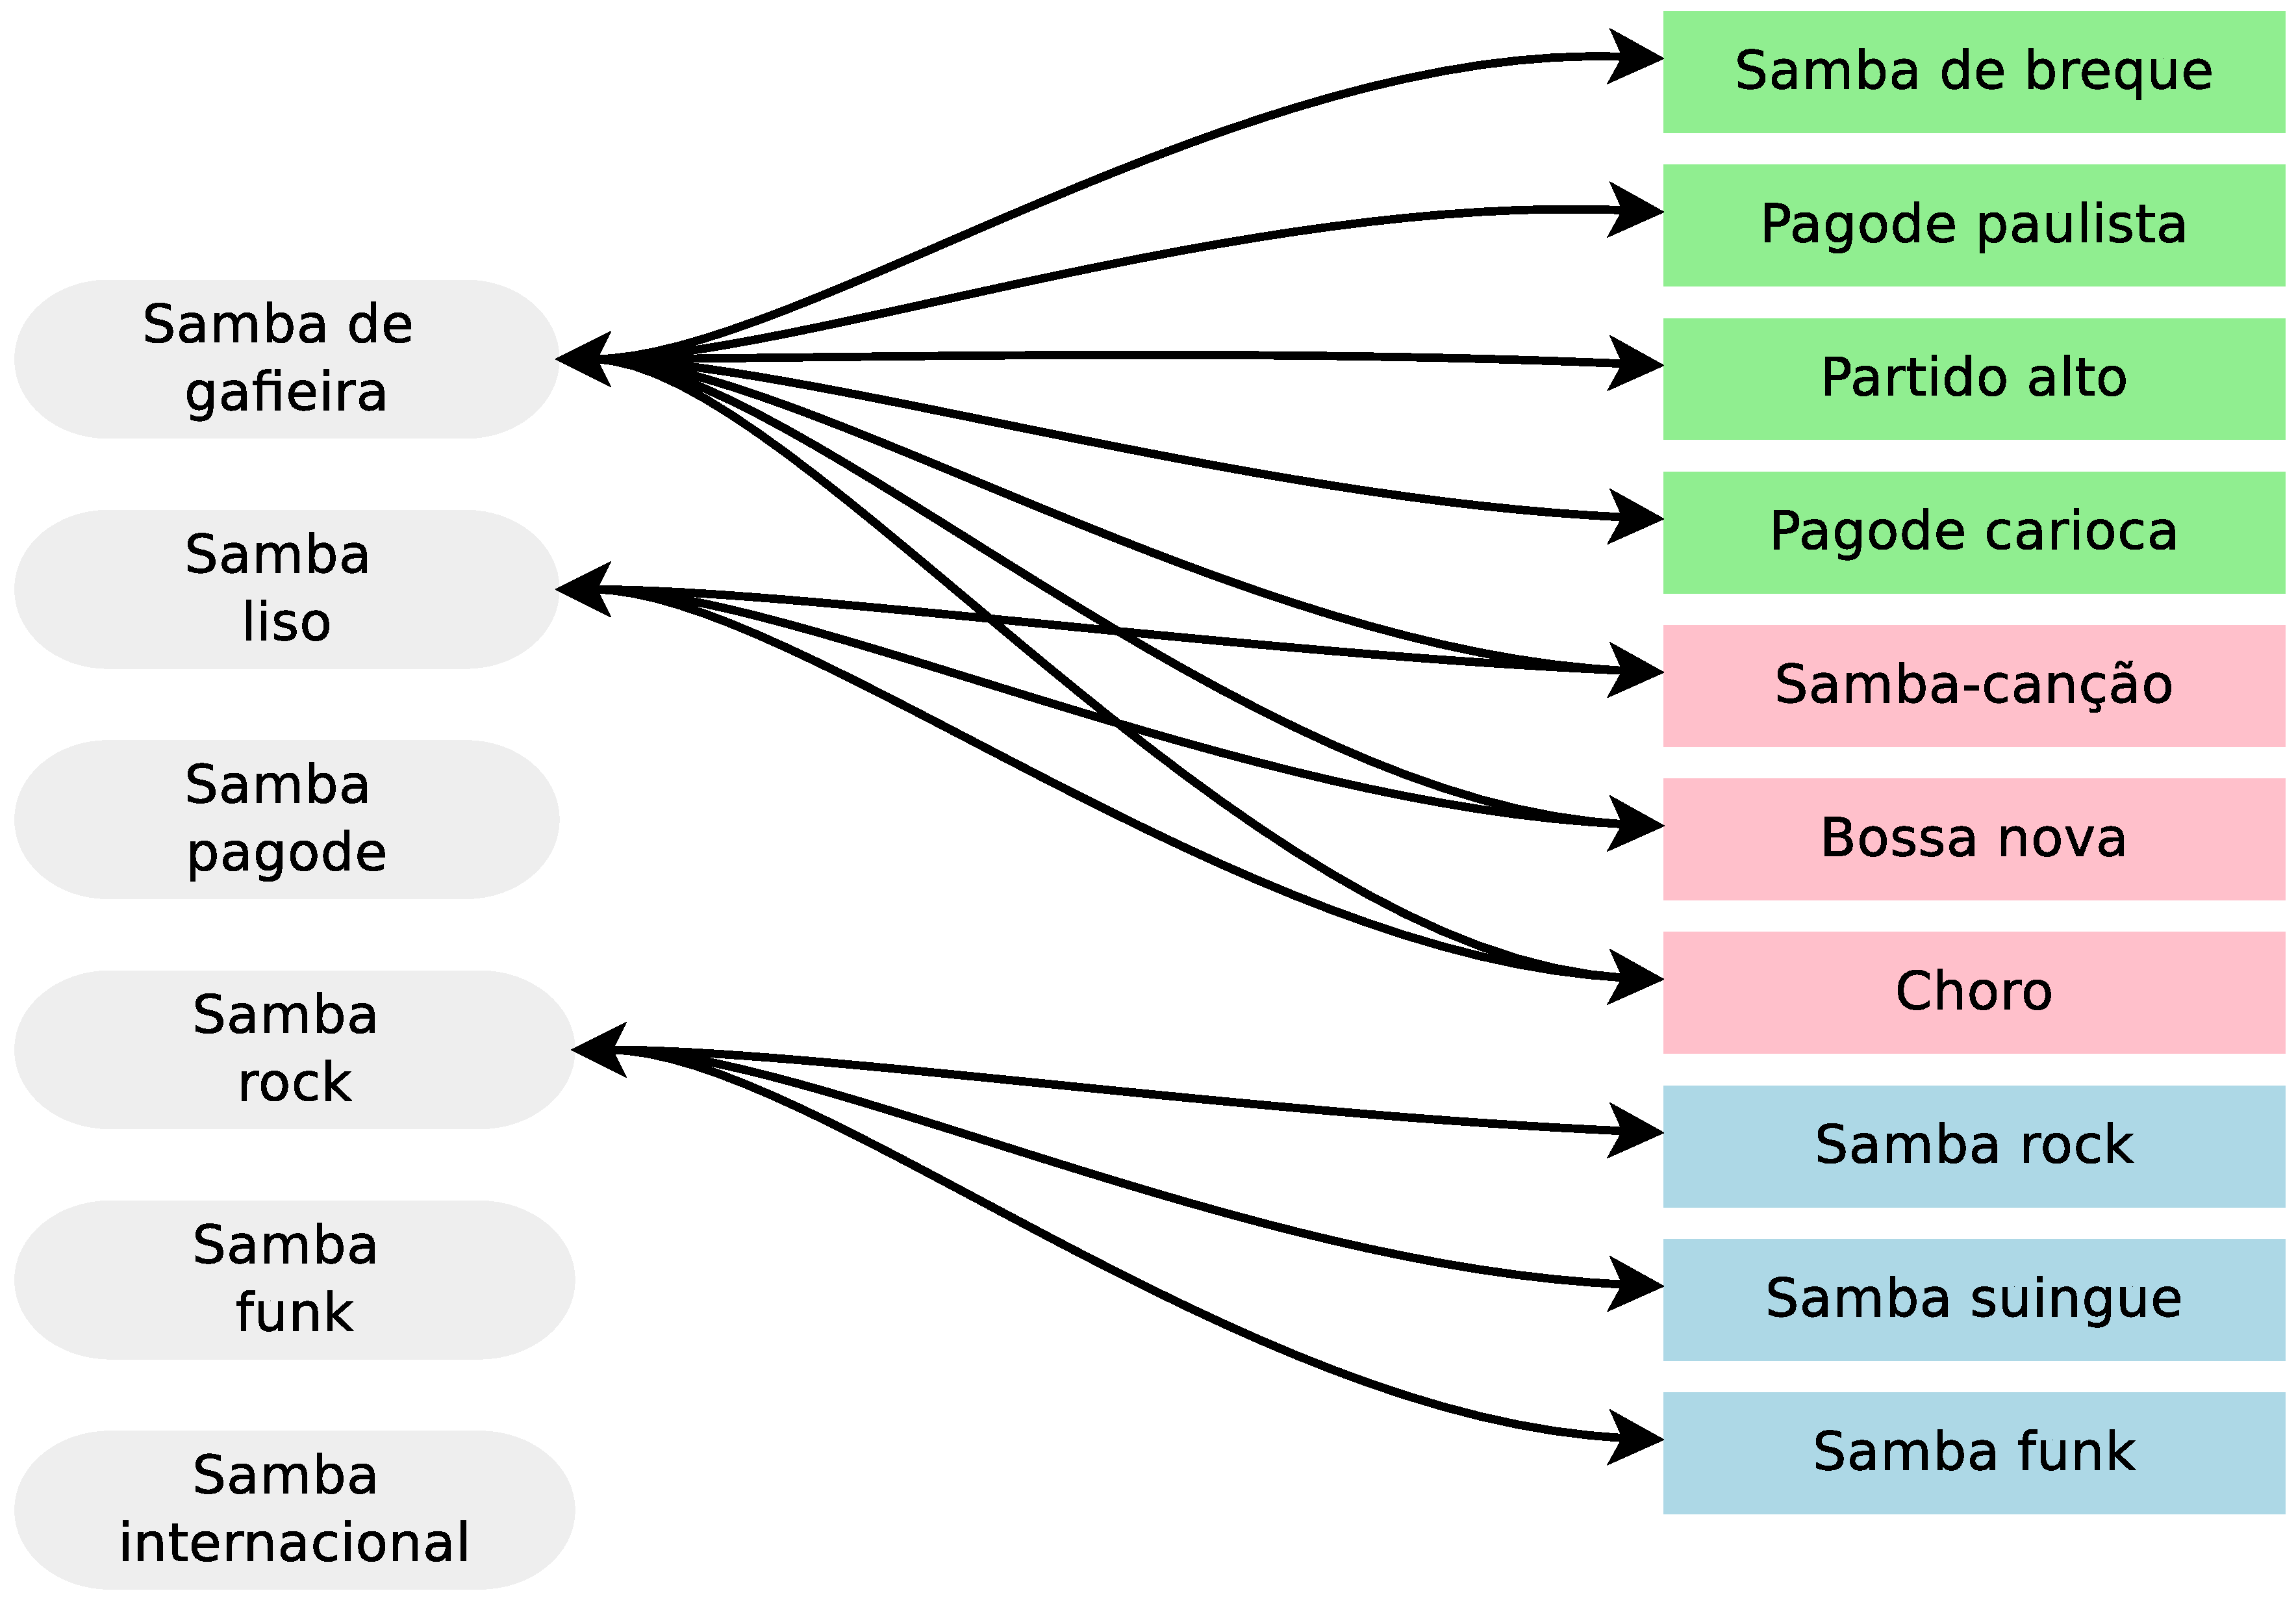
\includegraphics[width=0.6\textwidth]{chapters/cap-historia/dancavcmusica.eps}
  \caption{Relações entre os estilos de dança a dois e estilos de músicas no samba.}
\label{fig:sambadavavsmusica}
\end{figure}


Entre os estilos que se dançam de forma separada temos \cite[pp. 134]{perna2002samba}:
\begin{description}
\item[Samba reggae  (dança):] Este estilo de samba se dança separado, 
é uma dança baiana também conhecida como axé-dance, samba baiano ou pagode baiano,
se dança em samba reggae (música) \cite[pp. 134]{perna2002samba}.

\item[Samba no pé:] É o estilo usado nas quadras das escolas de samba,
se dança bem em estilos musicais como: 
camba enredo ou em qualquer samba rápido  \cite[pp. 134]{perna2002samba}.

\item[Marcha de carnaval:] É uma dança própria do carnaval para se dançar em cordões.
se dança bem em: marchas, marchas-rancho e samba-enredo lentos  \cite[pp. 135]{perna2002samba}.

\end{description}

Figura \ref{fig:sambadavavsmusicaseparado} \cite[pp. 134-138]{perna2002samba}

\begin{figure}[h]
  \centering
    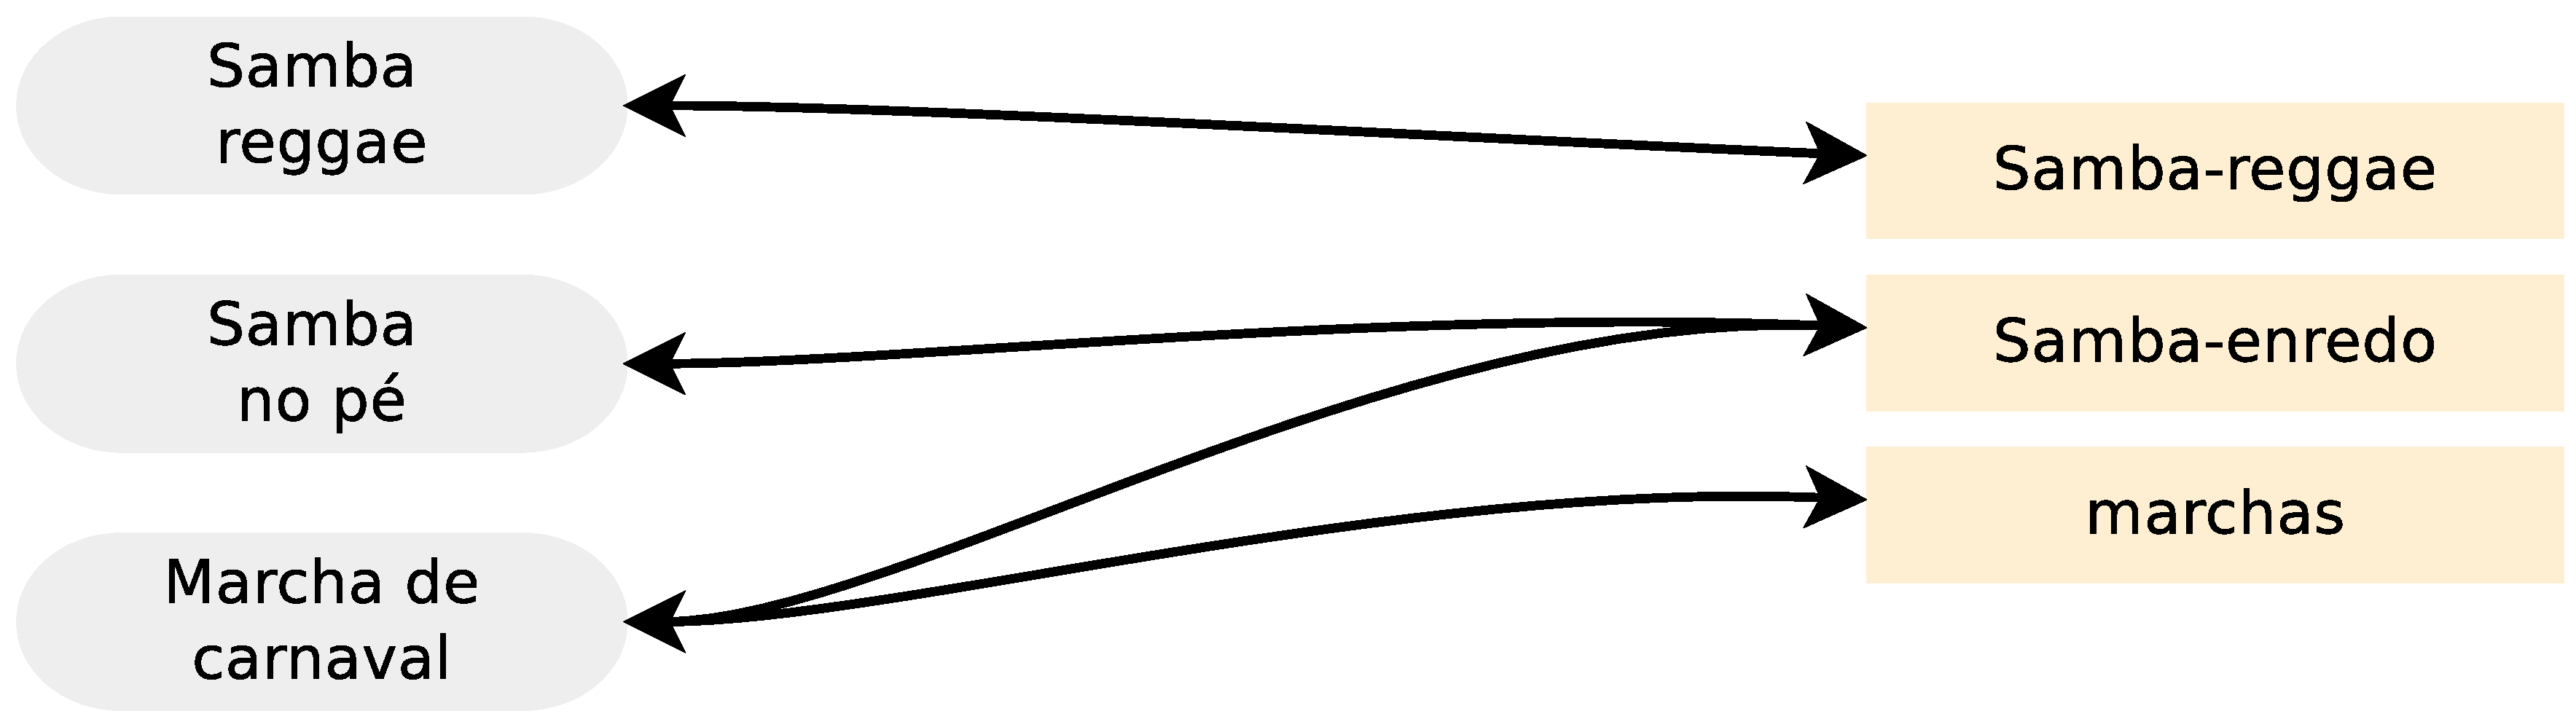
\includegraphics[width=0.6\textwidth]{chapters/cap-historia/dancavcmusicaseparado.eps}
  \caption{Relações entre os estilos de dança (separados) e estilos de músicas no samba.}
\label{fig:sambadavavsmusicaseparado}
\end{figure}
